% \chapter{Bayesian}
\section{Naive Bayes}
\label{sec:naive_bayes}

  In this section, we discuss how to classify vectors of discrete-valued features $\mathbf{x}$. Recall that we discussed how to classify a feature vector $\mathbf{x}$ by applying Bayes rule to a generative classifier of the form 
  $$p(y=c|\mathbf{x},\boldsymbol{\theta})\propto p(\mathbf{x}|y=c, \boldsymbol{\theta})p(y=c|\boldsymbol{\theta})$$
  The key to using such models is specifying a suitable form for the class-conditional density $p(\mathbf{x}|y=c, \boldsymbol{\theta})$, which defines what kind of data we expect to see in each class. 
  \begin{itemize}
    \item  $\textbf{x} \in \{1,...,K\}^D$,
    \begin{itemize}
      \item $K$: the number of values for each feature.
      \item $D$: the number of features.
    \end{itemize}
    \item We will use a generative approach.
    \item Need to specify the class conditional distribution, $p(\mathbf{x}|y=c)$.
    \item A simple approach is to assume the features are \textbf{conditionally independence} given the class label.
		\begin{figure}[h]
			\centering
			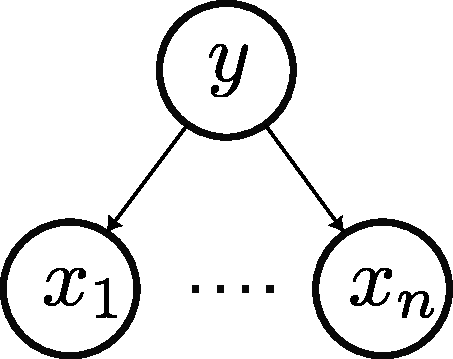
\includegraphics[scale=0.5]{./images/conditional_independence.pdf}
		\end{figure}
    \item This allows us to write the class conditional density as a product of one dimensional densities:
    $$p(\mathbf{x}|y=c, \boldsymbol{\theta}) = \prod_{j=1}^{D}p(x_j|y=c,\boldsymbol{\theta}_{jc})$$
  \end{itemize}
  The resulting model is called a \textbf{naive Bayes classifier (NBC)}. The model is called ``naive'' since we assume the independence between the features, which is not true in practice. However, if often results in classifiers that work well.

  The form of the class-conditional density depends on the type of each feature. We give some possibilities below:
  \begin{itemize}
    \item In the case of real-valued features, we can use the Gaussian distribution: $p(\mathbf{x}|y=c, \boldsymbol{\theta}) = \prod_{j=1}^{D}\mathcal{N}(x_j|\mu_{jc}^2)$, where $\mu_{jc}$ is the mean of feature $j$ in objects of class $c$, and $\sigma_{jc}^2$ is its variance.
    \item In the case of binary features, we can use the Bernoulli distribution: $p(\mathbf{x}|y=c, \boldsymbol{\theta}) = \prod_{j=1}^{D}\textrm{Ber}(x_j|\mu_{jc})$, where $\mu_{jc}$ is the probability that feature $j$ occurs in class $c$. This is sometimes called the \textbf{multivariate Bernoulli naive Bayes} model.
    \item In the case of categorical features, $x_j\in \{1,...,K\}$, we can model the multinomial distribution: $p(\mathbf{x}|y=c, \boldsymbol{\theta}) = \prod_{j=1}^{D}\textrm{Cat}(x_j|\mu_{jc})$, where $\boldsymbol{\mu}_{jc}$ is a histogram over the $K$ possible values for $x_j$ in class $c$.
  \end{itemize}

The probability for a single data case is given by
$$p(\mathbf{x}_i,y_i|\boldsymbol{\theta}) = p(y_i|\boldsymbol{\pi})\prod_{j}p(x_{ij}|\boldsymbol{\theta}_j)=\prod_{c}\pi_{c}^{\mathds{I}(y_i=c)}\prod_{j}\prod_{c}p(x_{ij}|\boldsymbol{\theta}_{jc})^{\mathds{I}(y_i=c)},$$
where $\boldsymbol{\pi}$ is a vector of class probability. Hence the log-likelihood is given by
	$$\textrm{log}p(\mathcal{D}|\boldsymbol{\theta}) = \sum_{c=1}^{C}N_c\textrm{log}\pi_c+\sum_{j=1}^{D}\sum_{c=1}^{C}\sum_{i:y_i=c}\textrm{log}p(x_{ij}|\boldsymbol{\theta}_{jc})$$

	\begin{algorithm}[H]
		\SetAlgoLined
%		\KwResult{Write here the result }
		Initialize $N_c=0,N_{jc}=0$ \;
		\For{$i=1:N$}{
      $c=y_i$ //Class label of $i$-th example;

      $N_c:=N_c+1$;

  		\For{$j=1:D$}{
      \uIf{$x_{ij}=1$}{
        $N_{jc}:=N_{jc}+1$
        }
  		}
		}
  $\hat{\pi}=\frac{N_c}{N},\hat{\theta}_{jc}=\frac{N_{jc}}{N_c}$
	\caption{Fitting a naive Bayes classifier to binary features}
\end{algorithm}
